\chapter{Durchführung der praktischen Untersuchungen}
\textbf{Kushagr Sinha}


Der experimentelle Teil lässt sich in zwei Versuche gliedern:

\begin{enumerate}
	\item \textbf{Lokalisation von Caspr2 an Synapsen:} Das Ziel war es,
	die Caspr2-Proteine sowohl an erregenden als auch an
	hemmenden Synapsen zu lokalisieren.
	\item \textbf{Einfluss von Caspr2-Antikörpern auf die
		Protein-Interaktion:} Spezifisch wurde untersucht, ob die
	Interaktion zum Protein Contactin-2 durch Caspr2-AK, gerichtet
	gegen die Discoidin- sowie Laminin1-Domänen, gestört wird.
\end{enumerate}

Um die Experimente beginnen zu können, wurden zunächst
Gehirnzellenkulturen, spezifisch Hippocampus-Neuronkulturen, benötigt. Dafür
werden aus einer trächtigen Maus die Embryonen entnommen, dekapitiert
und die Zellen aus der Hippocampus-Region des Gehirns entnommen.

Die Zelldichte ist so hoch, dass sie zu Ungenauigkeiten führen würde. Daher wurden die Zellen voneinander getrennt und verdünnt. Dafür
werden sie erst enzymatisch mit Trypsin behandelt, welches das Gewebe
lockert, damit diese beim Triturieren nicht zerquetscht werden.
Triturieren bezeichnet in diesem Zusammenhang das mechanische Vereinzeln
von Zellen durch Auf- und Abpipettieren der Gewebestücke.

Danach werden diese mit einer Zellsuspensionslösung versetzt und auf die
gewünschte Zelldichte verdünnt (ca.\ 20.000~Zellen/cm$^2$). Jetzt
werden die Zellen auf Deckgläschen verteilt, welche vorher mit
Poly-D-Lysin beschichtet wurden, um eine haftende Oberfläche für die
Zellen zu schaffen. Damit die Zellen dann auch ein neuronales Netzwerk
ausbilden, werden diese mit einem Neurobasal-Medium (NB), welches
Nährstoffe und Wachstumsfaktoren enthält, versetzt und anschließend 14~Tage
inkubiert.


% ────────────────────────────────────────────────────────────
\section{Untersuchung zur Lokalisation von Caspr2 an Synapsen}
% ────────────────────────────────────────────────────────────

Der gesamte Prozess zur Herstellung der Proben dauerte drei Tage.
Insgesamt wurden elf Proben hergestellt (siehe Tabelle~\ref{tab:proben}), welche
in verschiedene Versuchsgruppen unterteilt wurden. Am ersten Tag
befanden sich die Neuronzellen noch im NB, weswegen sie noch gewaschen,
also auf- und abpipettiert, werden mussten (siehe Abbildung \ref{fig:waschV}).
% (siehe Bild ?)
Dies wurde immer mit PBS (Phosphat-gepufferte Salzlösung) gemacht. Das
PBS wurde benutzt, da es eine isotonische, nicht-toxische Lösung ist,
die den pH-Wert stabilisiert und die Zellen schont.

Nachdem die Zellen dreimal gewaschen wurden, wurde ein Puffer~B1
aufgetragen, welcher aus 10\%iger BSA-Lösung (Rinderserumalbumin) und
10\%iger NDS-Lösung (normales Eselserum) bestand und als
Blockierungslösung diente. Ihr Zweck ist es, unspezifische
Bindungsstellen auf den Deckgläschen und in den Zellen zu besetzen. Dies
stellt sicher, dass die später hinzugefügten AK nur an ihre spezifischen
Zielproteine binden und kein störendes Hintergrundleuchten verursachen.

Nach einer Stunde Einwirkzeit wurde der Puffer~B1 abpipettiert und die
ersten Primärantikörper (Caspr2 bzw.\ der Kontrollantikörper)
hinzugefügt. Diese wurden anschließend über Nacht bei ungefähr vier Grad
inkubiert.

% ── Bild 1 ausgelassen ───────────────────────────────────────

\begin{table}[htbp]
	\centering
	
	\label{tab:proben}
	\begin{tabular}{c l c l c l}
		\toprule
		\textbf{Nr.} & \textbf{Färbung} &
		\textbf{Nr.} & \textbf{Färbung} &
		\textbf{Nr.} & \textbf{Färbung} \\
		\midrule
		(1)  & Caspr2 + VGlut1 &
		(5)  & Caspr2 + VGat   &
		(9)  & Control + VGlut1 \\
		(2)  & Caspr2 + VGlut1 &
		(6)  & Caspr2 + VGat   &
		(10) & Control + VGat \\
		(3)  & Caspr2 + VGlut1 &
		(7)  & Caspr2 + VGat   &
		(11) & negative control (nur SEK1+2) \\
		(4)  & Caspr2 + VGlut1 &
		(8)  & Caspr2 + VGat   &
		& \\
		\bottomrule
	\end{tabular}
	\caption{Übersicht der elf Proben und ihrer Versuchsgruppen.}
\end{table}
\clearpage
\begin{figure}[h]
	\centering
	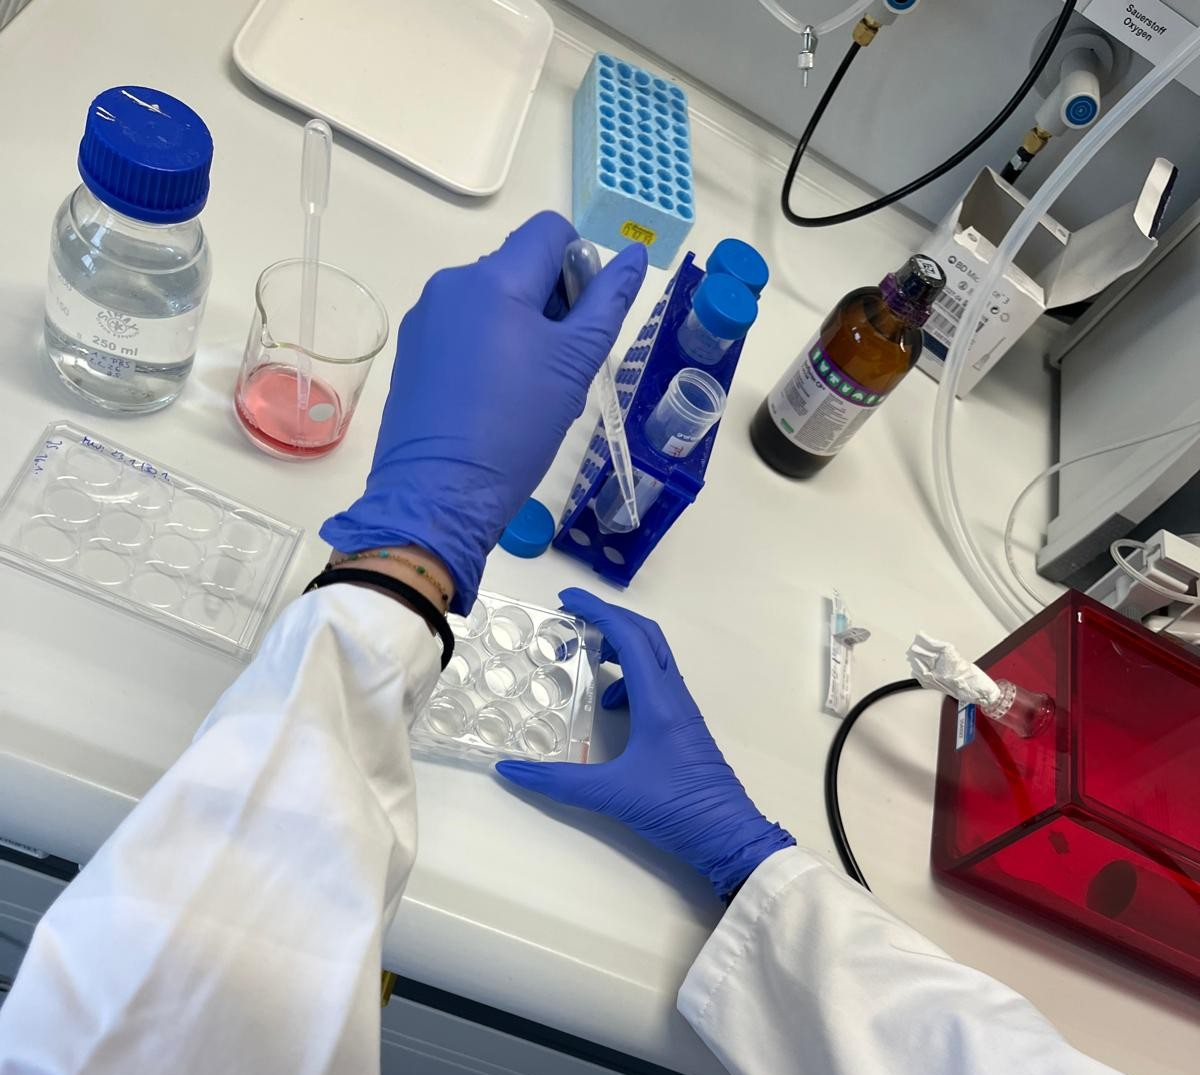
\includegraphics[width=0.8\textwidth]{abbildungen/waschvorgangDPU.jpeg}
	\caption{Vorgang des Waschen \parencite{eigenAu6.1}}
	\label{fig:waschV}
\end{figure}
Am zweiten Tag wurden die Deckgläschen in eine Feuchtekammer
transferiert. Dies ist notwendig, damit die geringen Mengen an
Antikörperlösung während der Einwirkzeit nicht verdunsten. Die Kammer
bestand aus einer Plastikbox mit angefeuchteten Papiertüchern als
Untergrund (siehe Abbildung \ref{fig:fKammer}).
% (siehe Bild 2)
\begin{figure}[h]
	\centering
	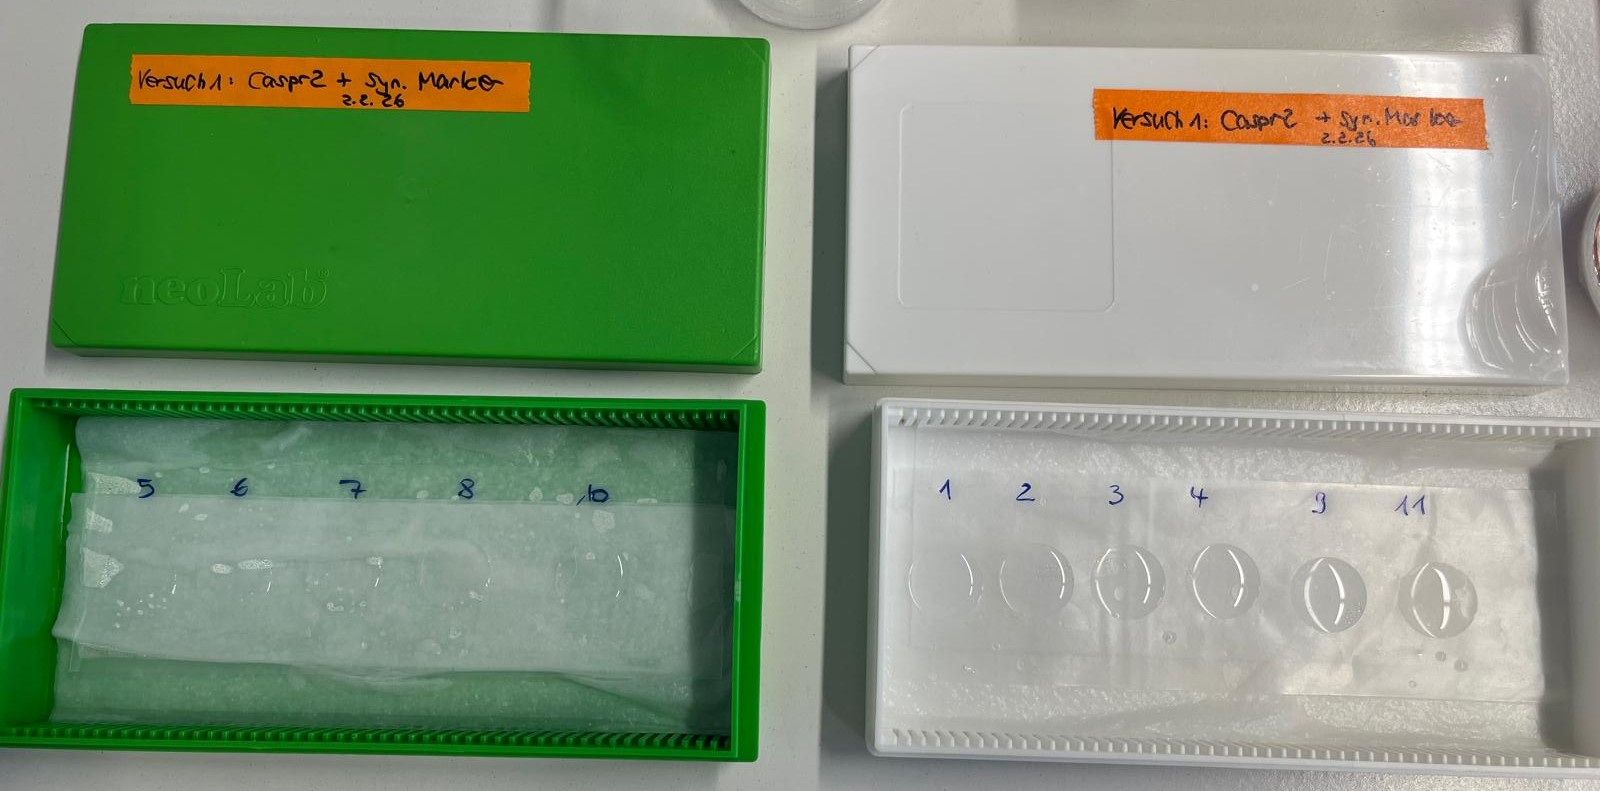
\includegraphics[width=1\textwidth]{abbildungen/fkammerDPU.jpeg}
	\caption{Feuchtekammer \parencite{eigenAu6.2}}
	\label{fig:fKammer}
\end{figure}

Nach sechsmaligem Waschen mit PBS wurden die ersten
Sekundärantikörper, nämlich AF647@sheep, dazugegeben. Bei der
Bezeichnung des Antikörpers wird angegeben: an erster Stelle, dass
dieser bei einer Wellenlänge von 647~nm leuchtet, und als Zweites, in
welchem Tier er gezüchtet wurde, also Schaf (sheep), passend zum ersten
Primärantikörper (Caspr2). Diese Lösung wurde nach zwei Stunden wieder
sechsmal abgewaschen.

Um die Zellen für die zweiten Primärantikörper besser zugänglich zu
machen, wurde eine Pufferlösung~B2 hergestellt. Diese bestand aus der
B1-Lösung und zusätzlich Triton. Das Triton dient dazu, kleine Löcher
in die Zellmembran zu machen, damit die VGlut/VGat-Antikörper auch in
das Innere der Synapse gelangen und binden können. Diese wurden nach der
Puffer-Behandlung hinzugefügt und erneut über Nacht bei 4\,°C gelagert.

Am dritten Tag wurde die Lösung wieder sechsmal mit PBS abgewaschen, und
es folgte die Zugabe der zweiten Sekundärantikörper, CF488@gp (leuchtet
grün und ist gerichtet gegen Meerschweinchen-AK) gegen VGlut- und
VGat-AK. Nach zwei Stunden wurde sechsmal abgewaschen.

Anschließend wurde DAPI hinzugefügt, eine Lösung, die den Zellkern
verfärbt, damit die Zellen unter dem Mikroskop besser erkannt werden
können.

Diese wurde dann dreimal gewaschen. Zehn Minuten lang wurden die
Präparate dann mit einer 4\%igen PFA-Lösung fixiert. Fixieren bedeutet,
die Proteine chemisch zu stabilisieren und die Zelle in ihrem aktuellen
Zustand \glqq einzufrieren\grqq{}, damit sie über Monate hinweg
mikroskopiert werden kann. Nach einem letzten Waschschritt waren die
Präparate fertig für die Auswertung.

\section{Untersuchung zur Einfluss von Caspr2-Antikörpern auf die
	Protein-Interaktion}